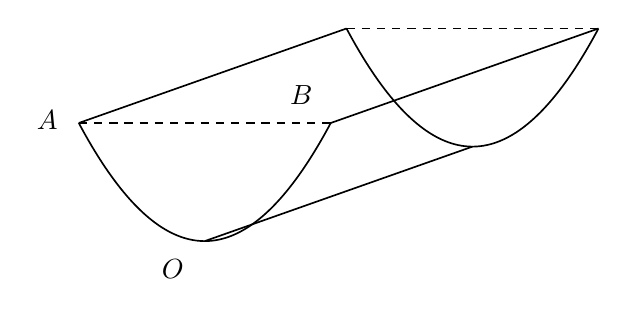
\begin{tikzpicture}[x=1cm,y=1cm,line width=.6pt,font=\normalsize,>=stealth,
  solid edge/.style={solid,line width=.6pt},
  hidden edge/.style={dashed,line width=.6pt,dash pattern=on 3pt off 2.5pt}]
% single trough: front parabola A-O-B, shifted back
\coordinate (Af) at (0.0,1.5);
\coordinate (Of) at (1.6,0.0);
\coordinate (Bf) at (3.2,1.5);
\coordinate (Ab) at (3.4,2.7);
\coordinate (Ob) at (5.0,1.2);
\coordinate (Bb) at (6.6,2.7);
% front parabola y=1.5x^2 mapped: A(-1,1.5)-O(0,0)-B(1,1.5) shifted to Af/Of/Bf
\draw[solid edge,domain=-1:1,samples=80] plot ({\x*1.6+1.6},{\x*\x*1.5});
% back parabola (visible right branch solid, hidden top dashed handled below)
\draw[solid edge,domain=-1:1,samples=80] plot ({\x*1.6+5.0},{\x*\x*1.5+1.2});
% longitudinal edges
\draw[solid edge] (Af)--(Ab);
\draw[solid edge] (Bf)--(Bb);
\draw[solid edge] (Of)--(Ob);
% width lines
\draw[hidden edge] (Af)--(Bf);
\draw[hidden edge] (Ab)--(Bb);
\node[left,xshift=-4pt,yshift=1pt] at (Af) {$A$};
\node[above left,xshift=-3pt,yshift=3pt] at (Bf) {$B$};
\node[below left,xshift=-4pt,yshift=-3pt] at (Of) {$O$};
\end{tikzpicture}
